\section{Integrais ( $\int$ )}

	\subsection{Integral Indefinida \cite{morettin}}

		\subsubsection{Definição \cite{morettin}}
	
			Chamamos de integral indefinida de $ g(x) $ e indicamos pelo símbolo $ \int g(x) \ dx $ a uma primitiva qualquer de $ g(x) $ adicionada a uma constante arbitrária $ c $. Assim:
			
			\bigskip
	
			{\LARGE $\int g(x)dx = f(x) + c $} \ ,
			
			\bigskip
	
			em que $ f(x) $ \footnote{Lucchesi \cite{lucchesi} utiliza a notação $ F(x) $ para representar funções primitivas.} é uma primitiva de $ g(x) $ , ou seja, $ f'(x) = g(x) $ \cite{morettin}
	
		\subsubsection{Funções Elementares \cite{morettin}}
	
			Podemos obter as integrais indefinidas das principais funções, que decorrem imediatamente das respectivas regras de derivação:
	
			\begin{enumerate}[label=(\alph*)]

				\item Se $ n $ é inteiro e diferente de $ -1 $ , então {\LARGE $\int x^{n} dx = \cfrac {x^{n + 1}} {n+1} + c $} , pois a derivada de $ \cfrac {x^{n + 1}} {n+1} $ é $ x^{n} $ .

				\item $\int \cfrac {1} {x} \ dx = \ln x + c $ , para $ x > 0 $ , pois a derivada de $ \ln x $ é $ \cfrac {1} {x} $ .
			
				observemos que se $ x < 0 $ , $ \int \cfrac {1} {x} \ dx = \ln (-x) + c $ . Assim, de modo geral, podemos escrever:

				\bigskip

				{\LARGE $\int \frac {1} {x} \ dx = \ln |x| + c$} .

				\item Para qualquer real $\alpha \neq -1$ , {\Large $\int x^{a} \ dx = \cfrac {x^{\alpha + 1}} {\alpha + 1} + c$} . \ $(x > 0)$
			
				\item {\LARGE $\int \cos xdx = \sin x + c$} , pois a derivada de $ \sin x $ é $ \cos x $ .

				\item {\LARGE $\int \sin xdx = - \cos x + c$} , pois a derivada de $- \cos x$ é $\sin x$ .

				\item {\LARGE $\int e^{x} \ dx = e^{x} + c$} , pois a derivada de $e^{x} $ é $e^{x}$ .

				\item {\LARGE $\int \cfrac {1}{1+x^{2}} \ dx = \arctan x + c$} , pois a derivada de $\arctan x$ é $\cfrac {1}{1+x^{2}}$ .

				\item {\LARGE $\int \cfrac {1}{\sqrt{1 - x^{2}}} \ dx = \arcsin x + c$} , pois a derivada de $\arcsin x$ é $\cfrac {1}{\sqrt{1 - x^{2}}} $ , para $ -1 < x < 1$ .
				
			\end{enumerate}
	
		\subsubsection{Propriedades Operatórias \cite{morettin}}
	
			\begin{enumerate}[label=(P\arabic*)]
			
				\item {\LARGE $\int [ f_{1} (x) + f_{2} (x) ] \ dx = \int f_{1} (x) \ dx + \int f_{2} (x) \ dx$} ;
			
				\item {\LARGE $\int [ f_{1} (x) - f_{2} (x) ] \ dx = \int f_{1} (x) \ dx - \int f_{2} (x) \ dx$} ;
			
				\item {\LARGE $\int c \cdot f(x) \ dx = c \cdot \int f(x) \ dx$} .
		
			\end{enumerate}
	
	\subsection{Integral Definida \cite{morettin}}

		\subsubsection{Definição \cite{morettin}}
	
			Seja $ f(x) $ uma função e $ g(x) $ uma de suas primitivas. Portanto, $ \int f(x) \ dx = g(x) + c $ .

			Definimos a integral definida de $ f(x) $ entre os limites $ a $ e $ b $ como a diferença $ g(b) - g(a) $ , e indicamos simbolicamente
			
			\bigskip

			{\LARGE $ \int_{a}^{b} f(x) \ dx = g(b) - g(a) = \lim \limits_{x \to b-} [g(x)] - \lim \limits_{x \to a+} [g(x)] $} .

			\bigskip

			A diferença $ g(b) - g(a) $ também costuma ser indicada pelo símbolo $ [g(x)]_{a}^{b} $.
	
		\subsubsection{Teorema Fundamental do Cálculo \cite{morettin}}
	
			O significado geométrico da integral definida é dado a seguir.

			Seja $ f(x) $ uma função \textbf{contínua e não negativa} definida num intervalo $ [a, b] $ . A integral definida $ \int_{a}^{b} f(x) \ dx $ representa a área da região compreendida entre o gráfico de $ f(x) $ , o eixo $ x $ e as verticais que passam por $ a $ e $ b $ .

			\bigskip

			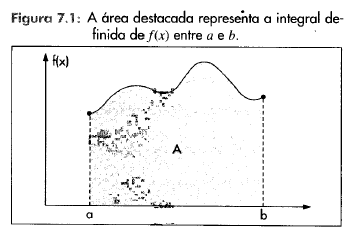
\includegraphics[height=6cm]{images/morettin_figura-7-1}

			Assim, indicado por \textbf{$ A $} a área destacada da Figura 7.1, teremos:
			
			\bigskip

			{\LARGE $A = \int_{a}^{b} f(x) \ dx$}
	
			\bigskip
			
			(...) Caso $ f(x) $ seja negativa no intervalo $ [a, b] $ , a área $ A $ da região delimitada pelo gráfico de $ f(x) $ , eixo $ x $ , e pelas verticais que passam por $ a $ e por $ b $ é dada por:

			\bigskip

			{\LARGE $A = - \int_{a}^{b} f(x) \ dx$} .

		\subsubsection{Propriedades Operatórias \cite{lucchesi}}
		
			\begin{enumerate}[label=(P\arabic*)]
			
				\item {\Large $\int_{a}^{a} f(x) \ dx = F(a) - F(a) = 0$}
				
				\item {\Large $\int_{a}^{b} f(x) \ dx = - \int_{b}^{a} f(x) \ dx$}
			
				\item {\Large $\int_{a}^{b} f(x) \ dx = \int_{a}^{c} f(x) \ dx + \int_{c}^{b} f(x) \ dx $} , sendo $ a < c < b$ .
		
			\end{enumerate}
	
	\subsection{Integral Imprópria \cite{lucchesi}}
	
		\subsubsection{Definição \cite{lucchesi}}
	
			Quando as hipóteses do teorema fundamental do cálculo falharem, aplicamos a integral imprópria.
		
			Caso 1: Intervalo de integração aberto (e.g. ]a, b]).
			
			Caso 2: Descontinuidade da função (e.g. $ D = \mathbb{R} - (0) $ ).
		
			Usa-se a propriedade da integral definida:
		
			\begin{enumerate}[label=(P3)]
			
				\item {\LARGE $\int_{a}^{b} f(x) \ dx = \int_{a}^{c} f(x) \ dx + \int_{c}^{b} f(x) \ dx $ , sendo $ a < c < b $} .
		
			\end{enumerate}

			\medskip		

			\textbf{Exemplo}:

				\medskip

				$\int_{-1}^{1} \frac {1}{x^2} \ dx \ \longrightarrow \ D = \mathbb{R} - (0) $
			
				\bigskip
			
				$ \int_{-1}^{1} \frac {1}{x^2} \ dx = \lim \limits_{z \to 0^{-}} \int_{-1}^{z} \frac {1}{x^2} \ dx + \lim \limits_{z \to 0^{+}} \int_{z}^{1} \frac {1}{x^2} \ dx $